\section{Introducción}
\subsection{Bin Packing Problem (BPP)}
El Bin Packing Problem (BPP), o problema de empacado en contenedores, consiste en asignar un conjunto de objetos (paquetes) de diferentes tamaños 
buscando un número mínimo de contenedores con capacidad limitada. Tanto los objetos como los contenedores se 
consideran homogéneos: cada objeto posee un tamaño $p_i > 0$ y cada contenedor tiene una capacidad fija $C$.  
Debido a la naturaleza combinatoria del problema, el BPP es considerado NP-hard, por lo que resolverlo de manera exacta se vuelve inviable 
a medida que el número de objetos crece.

\subsection{Técnicas de optimización inspiradas en procesos naturales}

En las últimas décadas, muchos problemas complejos de optimización han sido abordados mediante algoritmos inspirados en procesos naturales. 
Estos métodos imitan comportamientos observados en la biología, la física y la ecología, permitiendo explorar grandes espacios de búsqueda 
de forma eficiente sin requerir una solución exacta.

Entre las técnicas más comunes se encuentran:

\begin{itemize}
    \item \textbf{Optimización por Enjambre de Partículas (PSO):} Modela el movimiento colectivo de bandadas de aves o bancos de peces, 
                actualizando las soluciones mediante la experiencia individual y colectiva.
    \item \textbf{Recocido Simulado (SA):} Inspirado en el proceso físico de enfriamiento del metal, explora soluciones aleatorias 
                permitiendo aceptar temporalmente soluciones peores para evitar óptimos locales.
    \item \textbf{Sistemas Inmunes Artificiales (AIS):} Simulan la adaptación del sistema inmunológico, identificando patrones, clonando 
                buenas soluciones y descartando respuestas ineficientes.
\end{itemize}

Estas técnicas, conocidas como metaheurísticas, son especialmente útiles para problemas NP-hard, donde la búsqueda exhaustiva es impráctica. 
Entre ellas, uno de los métodos más efectivos para problemas combinatorios es la Ant Colony Optimization (ACO).

\subsection{Ant Colony Optimization aplicada al Bin Packing}

El metodo de Ant Colony Optimization (ACO), propuesta originalmente por Dorigo y colaboradores~\cite{dorigo1996ant, dorigo2006ant}, 
es una metaheurística inspirada en la forma en que las hormigas reales encuentran rutas óptimas entre su colonia y una fuente de alimento. 
Su mecanismo central se basa en el uso de feromonas, una señal química que marca rutas prometedoras; conforme más hormigas utilizan un 
camino, mayor es la cantidad de feromona acumulada, reforzando su probabilidad de ser elegido nuevamente.

En el contexto del Bin Packing Problem (BPP), cada hormiga construye una solución asignando objetos a contenedores siguiendo un proceso 
probabilístico que combina dos fuentes de información:

\begin{enumerate}
    \item \textbf{La feromona} almacenada para cada combinación objeto–contenedor, que refleja qué tan útil ha sido esta asignación en 
                soluciones previas.
    \item \textbf{La heurística}, que evalúa localmente la conveniencia de colocar un objeto en un contenedor, típicamente basada en el 
                espacio restante.
\end{enumerate}

La probabilidad de que una hormiga $k$ asigne el objeto $i$ al contenedor $j$ viene dada por:

\begin{equation}
P_{ij}^{(k)} = 
\frac{\tau_{ij}^{\alpha} \, \eta_{ij}^{\beta}}
{\sum\limits_{l \in \text{Contenedores válidos}} \tau_{il}^{\alpha} \, \eta_{il}^{\beta}},
\label{eq:probabilidad}
\end{equation}

donde:

\begin{itemize}
    \item $\tau_{ij}$ es la cantidad de feromona asociada a asignar el objeto $i$ en el contenedor $j$.
    \item $\eta_{ij}$ es la heurística, por ejemplo: 
    \begin{equation}\label{eq: heuristica}
    \eta_{ij} = \frac{1}{1 + \text{espacio restante en el contenedor } j}
    \end{equation}
    favoreciendo contenedores cuyo espacio sobrante sea pequeño (mejor llenado).
    \item $\alpha$ controla la \textbf{importancia de la feromona}.  
    \item $\beta$ controla la \textbf{importancia de la heurística}.  
\end{itemize}


\subsubsection*{Evaporación y depósito de feromonas}

Las feromonas evolucionan dinámicamente en cada iteración.  
Primero ocurre la \textbf{evaporación}, que evita que soluciones viejas dominen indefinidamente:

\begin{equation}
\tau_{ij} \leftarrow (1 - \rho) \, \tau_{ij},
\label{eq:evaporacion}
\end{equation}

donde $\rho$ es la \textit{tasa de evaporación}.  
En nuestro caso, $\rho = 0.5$ implica que la mitad de la feromona se pierde en cada iteración, lo que mantiene la exploración activa.

Después de que todas las hormigas han construido sus soluciones, se deposita feromona adicional en las asignaciones que pertenecen a la mejor solución de la iteración o a la mejor global:

\begin{equation}
\tau_{ij} \leftarrow \tau_{ij} + \Delta \tau_{ij},
\end{equation}

donde la cantidad añadida sigue el esquema clásico:

\begin{equation}
\Delta \tau_{ij} = 
\begin{cases}
\displaystyle \frac{Q}{f_{\text{best}}}, & \text{si el objeto $i$ fue asignado al contenedor $j$ en la mejor solución}, \\
0, & \text{en otro caso},
\end{cases}
\label{eq:deposito}
\end{equation}

y $f_{\text{best}}$ es el valor de la función de aptitud de la mejor hormiga.  
El parámetro $Q$ determina cuánta feromona se deposita; al usar $Q = 1.0$, el refuerzo es proporcionalmente moderado y estable.

\subsubsection*{Interpretación en el Bin Packing}

En este modelo:

\begin{itemize}
    \item Una asignación que contribuye a llenar mejor los contenedores recibe más feromona.
    \item La heurística ($\beta = 2.0$) tiene mayor peso que la feromona, favoreciendo decisiones inmediatas basadas en el espacio restante.
    \item La evaporación ($\rho = 0.5$) mantiene un equilibrio entre exploración y explotación.
\end{itemize}

Así, las hormigas no solo siguen caminos exitosos, sino que también exploran nuevas combinaciones de asignación, permitiendo gradualmente 
encontrar configuraciones más eficientes de empacado.

\subsection{Problema}
Para este trabajo considerademos 5 contenedores, de la A a la E, cada uno con capacidad 6 y 7 paquetes con tamaños variados que deben ser 
asignados a estos contenedores.

\begin{figure}[H]
    \centering
    \includegraphics[width=0.6\textwidth]{rsc/img/intro/Bin_Packing.png}
    \caption{Representación del problema de empacado en contenedores.}\label{fig:bin_packing}
\end{figure}

Ejemplos de forma de acomodar los paquetes en los contenedores.
\begin{figure}[H]
    \centering
    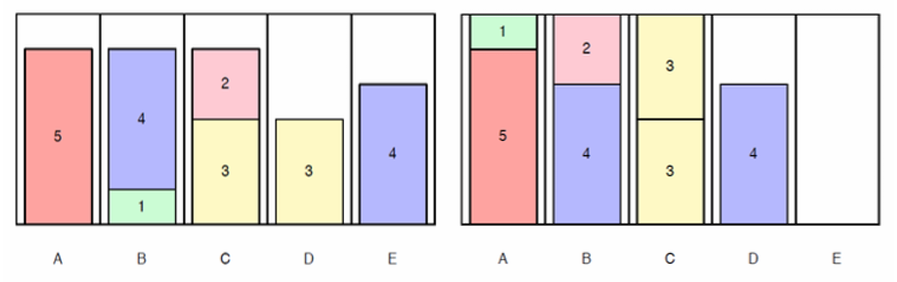
\includegraphics[width=0.6\textwidth]{rsc/img/intro/ejemplos.png}
    \caption{Ejemplos de formas de acomodar los paquetes en los contenedores.}\label{fig:ejemplos}
\end{figure}